\section{Theoretical framework} \label{theoreticalframework}
The goal of the theoretical framework is to summarise the existing knowledge on the subjects related to the (main)research question. These questions define the scope of the theoretical framework:
\begin{itemize}[label={}]
\item \tfone
\item \tftwo
\item \tfthree
\item \tffour
\item \tffive
\end{itemize}
%=================================================================================================================================================================================================

\subsection{Decision making: science or art?} \label{tf_ebm}
We typically use prior experience, intuition, or advice from others to make decisions \parencite{DM12}. However, making a professional decision that might impact colleagues and customers is typically more challenging. We need to convince our stakeholders with the right arguments. Evidence-based management classifies these arguments. \cite{DM03} define evidence-based management as:
\begin{quote}\itshape
"Making decisions through the conscientious, explicit, and judicious use of four sources of information: practitioner expertise and judgment, evidence from the local context, a critical evaluation of the best available [external]research evidence, and the perspectives of those people who might be affected by the decision." \parencite{DM03}
\end{quote}

\subsubsection{Decision-making model} \label{tf_dmm}
Figure \ref{fig:dmm01} presents a mixed-level model for evidence-based decision-making. This model shows that a decision-maker bases a decision on multiple evidence types. The size of the circle represents the amount of influence the evidence type has in a specific decision.

\begin{figure}[H]
\centering
  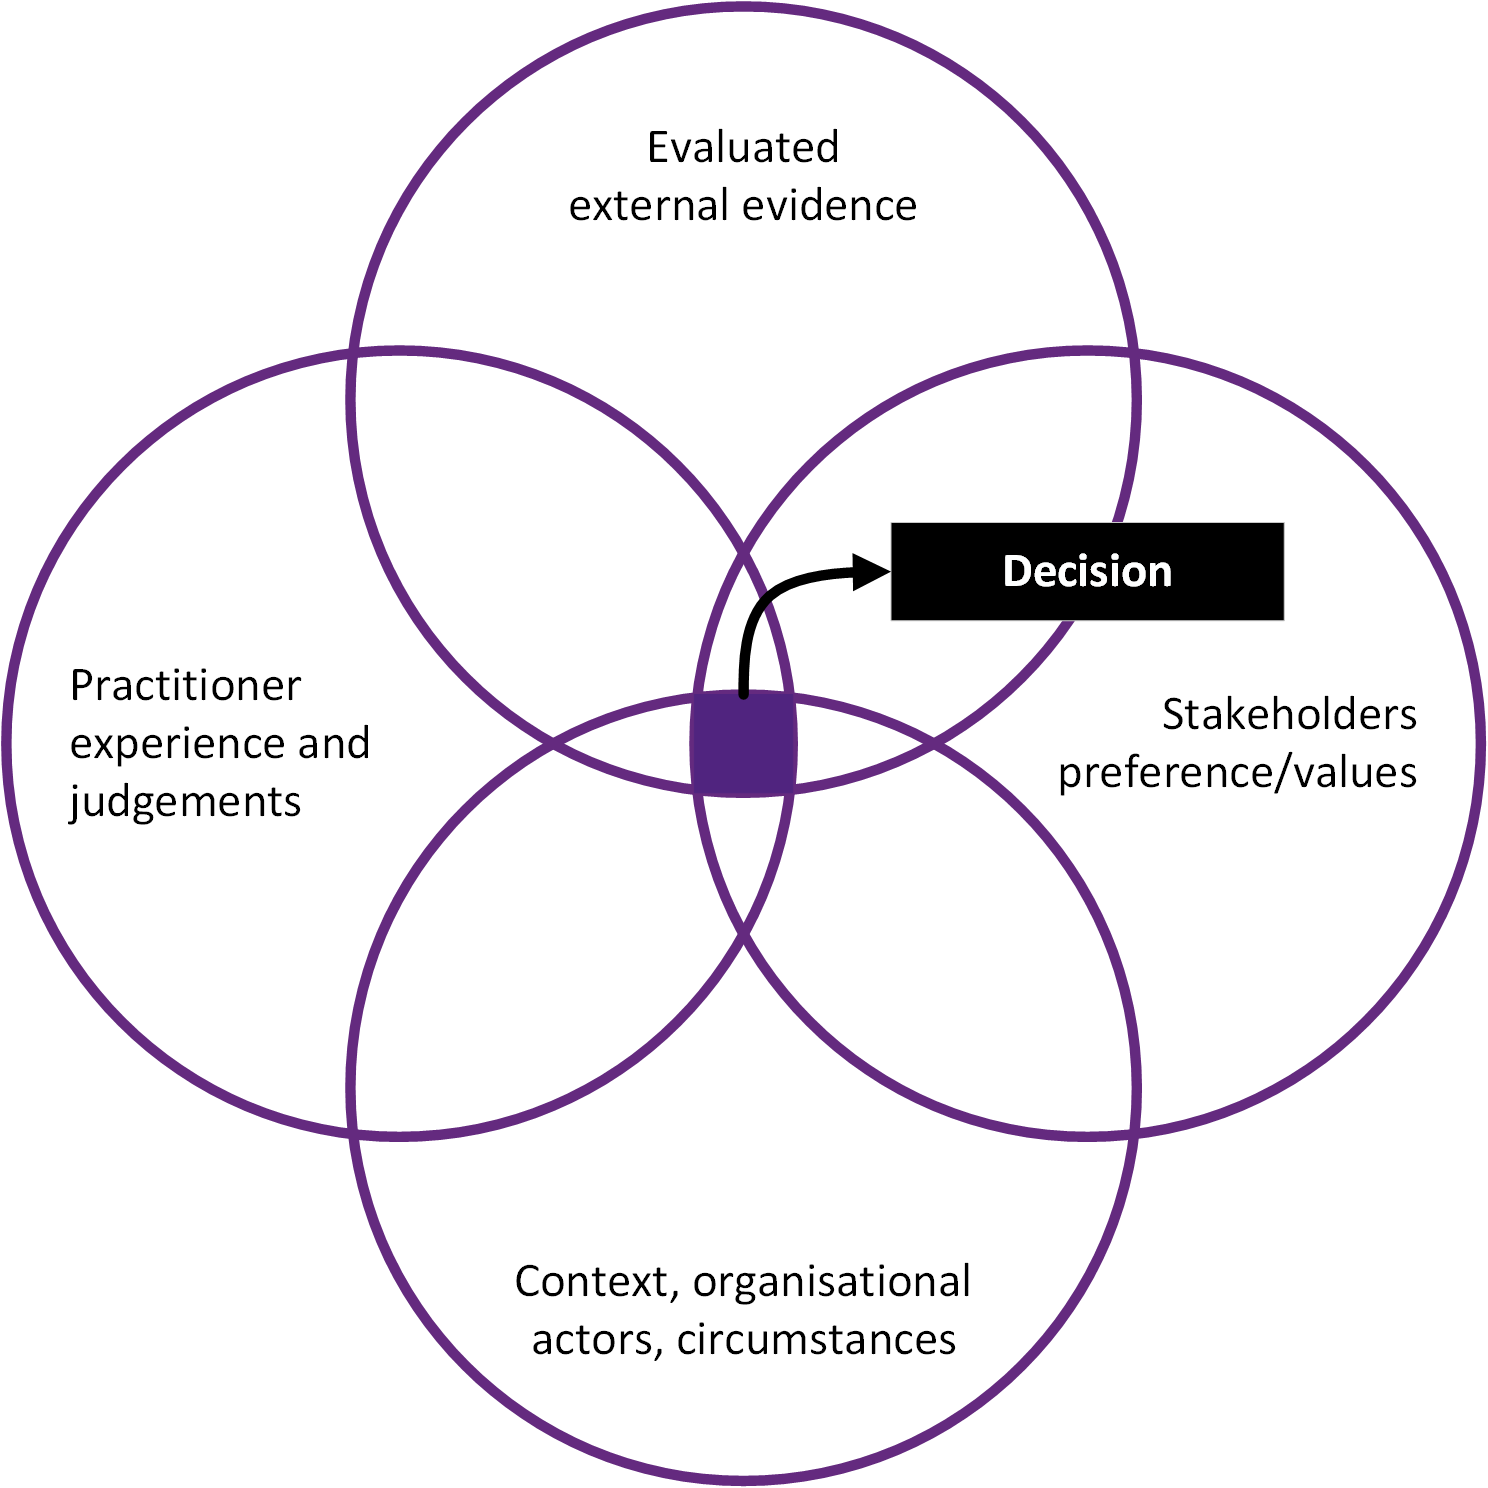
\includegraphics[width=8cm]{../../Images/DM07_Evidence.png}
  \caption{The four elements of evidence-based management \parencite{DM03}. The size of each circle (representing the strength of its influence) varies with each decision. For example, if we move the context, organisational actors, and circumstances further to the bottom, its influence in the decision decreases.}
  \label{fig:dmm01}
\end{figure}

Evidence includes local context\footnote{The context for individuals is given by the organisation and the context for the organisation is given by the external environment \parencite{DM04}.}, insight from other sources, and professional experience (or \textit{"accumulated past experience"} \parencite{PM04}) \parencite{DM03}. Different people use evidence types in different ways, depending on their personal experience. \cite{DM07} argue that evidence-based decision making is influenced by:
\begin{quoting}\itshape
"[...] managers' preferences and values as well as stakeholders' preferences within institutional, organisational and individual contexts." \parencite{DM07}.
\end{quoting}

Evidence-based decision-making considers the way decision-makers gather the evidence, ensure this suits the usage of the evidence (methodological fit), and the context in which the information used \parencite{DM07}. The quality of the information depends on its reproducibility, the transparency on evidence conflicts, and the consensus of evidence.

\subsubsection{Technology-driven knowledge management}
A knowledge management strategy represents how organisations have implemented knowledge management and how it impacts the firm's decision making \parencite{KM03}. The knowledge management strategy approach structures organisational knowledge to justify strategic choices (or decisions) and can save time in the decision-making process. 

%=================================================================================================================================================================================================
\subsection{Detecting premature information}
We use Semantic Web technologies to detect premature information. 

\subsubsection{Resource description framework schema (RDFS)}
Linking information starts with creating a \emph{common understanding} of the data concepts between different contexts: this is the goal of the Resource Description Framework (RDF) \parencite{SM13}. RDF Schema (RDFS) provides data-modelling mechanisms on top of RDF, allowing it to describe groups of related resources and the relationships between those resources \parencite{WEB06}. 

\subsubsection{SPARQL Query Language for RDF}
The SPARQL query language can query data stored in an RDFS data model. SPARQL can be considered a data-access and filtering protocol for RDFS \parencite{WEB08}. SPARQL uses a table to present its output (or result set). SPARQL can be used to test data in RDFS graphs by defining constraints in SPARQL and observing the output.

SPARQL queries can select data from an ontology. If a query returns with an empty result set, the constraints described in the $WHERE$ clause of query do not match any information in the ontology. This mechanism led to SPIN \parencite{WEB13}, also known as SPARQL rules. SPIN can attach SPARQL queries to classes. The SPARQL query would define the constraints that each instance of the class needs to satisfy. \cite{SM34} submitted SPIN to the W3C. However, SPIN never made it to a recommended standard. 

\subsubsection{Web Ontology Language}
The Web Ontology Language (OWL) can be used on top of RDF(S) to increase the expressivity in the relationships between data fields. Its main goal is to \emph{represent} knowledge \parencite{WEB04}. While RDF(S) describes the data and its relationships within a single ontology, OWL allows relationships between multiple ontologies and their data fields and supports various types of inference. Inferencing makes it easier to discover relationships between fields and reveal complexity in a structure that was not visible before \parencite{SM13}. 

The consistency on an OWL ontology can be checked by a reasoner, for example, Pellet. A reasoner includes consistency checkers based on the OWL specification \parencite{SM32}:
\begin{quote}\itshape
'An OWL consistency checker takes a document as input and returns one word being Consistent, Inconsistent, or Unknown.' \parencite{WEB12}
\end{quote}

Semantic web inferencing and reasoning works based on rules defined in OWL. The reasoner derives new facts from these rules. For example, the \emph{Super Property Of (Chain)} allows defining a chain of relationships; for example, $customer\_bought\_product\_from\_manufacturer$ is a combination of two relationships: $manufacturer\_produces\_product$ and $product\_bought\_by\_customer$. When these two relationships are defined, the reasoner automatically infers the super property (figure \ref{fig:superproperty}). Inferencing decreases the risk of mistakes and increases the completeness of the information. As a result, inferencing decreases the risk the decision-relevant information does not meet the expected requirements.

\begin{figure}[H]
\centering
  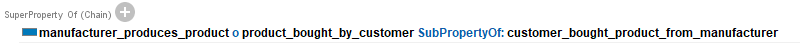
\includegraphics[width=17cm]{../../Images/Superproperty.png}
  \caption{A super property that defines a chain of object properties. For example, the super property $customer\_bought\_product\_from\_manufacturer$ relates manufacturers with customers using the object properties $manufacturer\_produces\_product$ and $product\_bought\_by\_customer$.}
  \label{fig:superproperty}
\end{figure}

\subsubsection{Semantic web rule language (SWRL)}
\cite{SM35} attempted to introduce data validation mechanisms in the context of the Semantic Web. SWRL extends OWL with Horn-like rules that are a form of implication between an antecedent and consequent: whenever the antecedent is true, the consequent should be true as well. SWRL never made it past its W3C submission state. Semantic Web reasoners are also able to infer new knowledge based on SWRL rules.

\subsubsection{Shapes constraints language (SHACL)} \label{tfshacl}
OWL suffers from restrictions related to the limited possibilities for structural validation, and the built-in nature of the so-called \emph{Open World Assumption}\footnote{The open world assumption prevents a negation as failure that means that the absence of information cannot lead to any conclusion, but results in an \emph{unknown} evaluation.} \parencite{SM22}. Another limitation of OWL relates to the way how restrictions are working. For example, a person \emph{p} can only have one father, but \emph{p} has two individuals defined as a father. OWL assumes that these two values are representing the same real-world entity.

The W3C has accepted SHACL (Shapes Constraint Language) as a recommendation in 2017 \parencite{WEB05} to address these limitations. The main goal of SHACL is the \emph{validation} of RDF(S) graphs against a set of conditions by defining SHACL shapes \parencite{WEB05}. Figure \ref{fig:shacl1} presents SHACL conceptually. SHACL can detect data quality issues \parencite{SM23} based on the definition of constraints. For example, each person needs to have precisely one last name.  

\begin{figure}[H]
\centering
  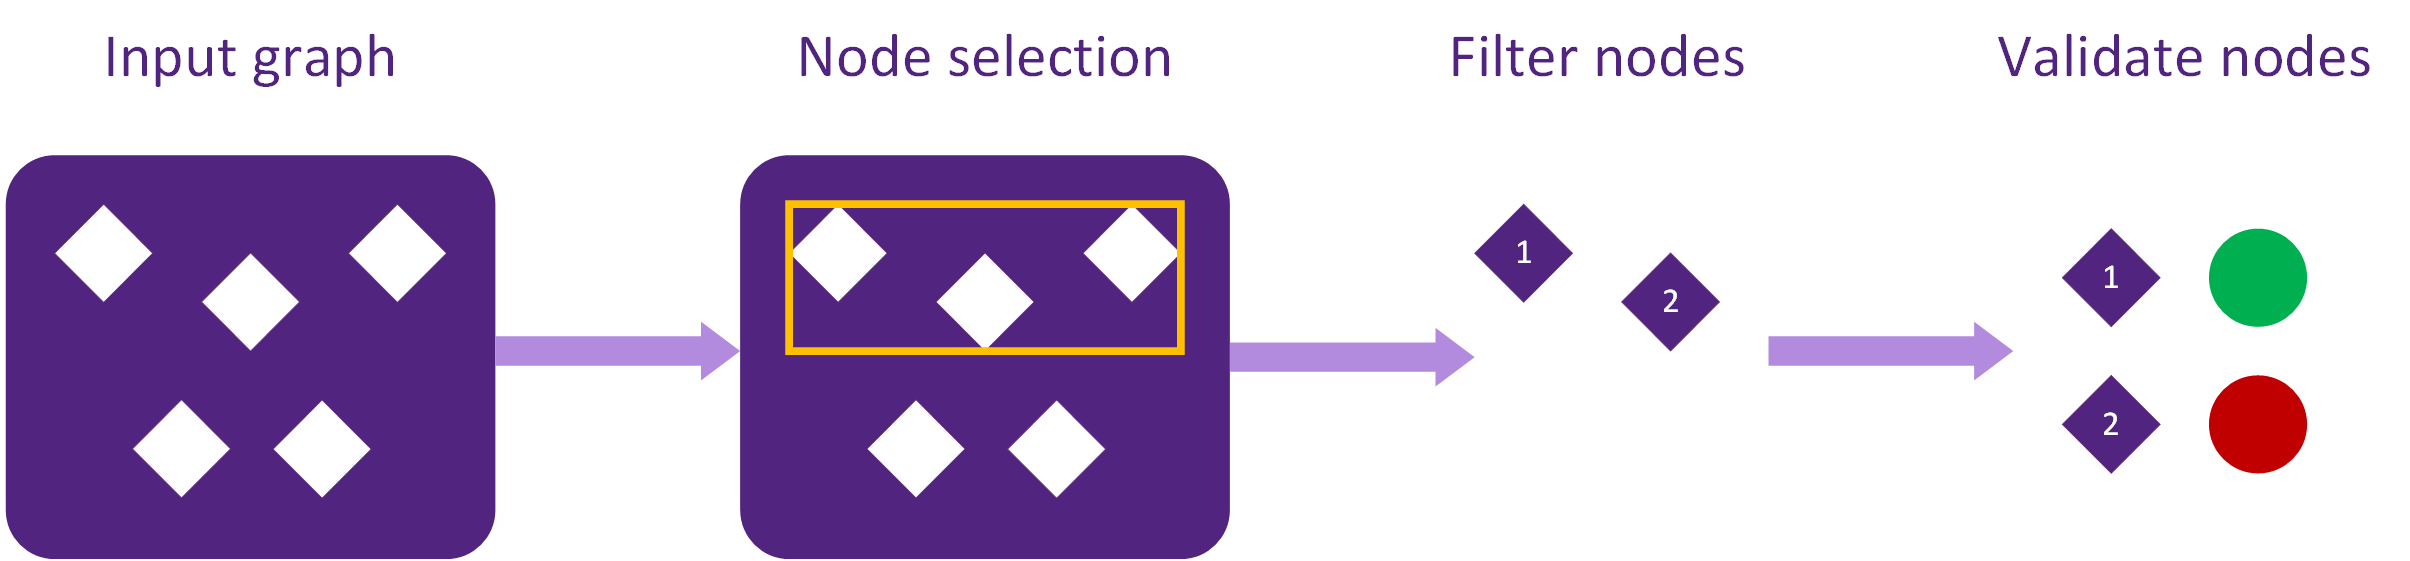
\includegraphics[width=15cm]{../../Images/SHACL1.png}
  \caption{The main goal of SHACL is the \emph{validation} of RDF(S) graphs against a set of conditions by defining SHACL shapes \parencite{WEB05}.}
  \label{fig:shacl1}
\end{figure}

%=================================================================================================================================================================================================
\subsection{Transformation of information into decisions} \label{tf_transformation_of_information}
The way a decision support system presents information to a user has a significant impact on the quality of that system \parencite{BI03}. Decision-makers can use the information as a communication medium, a knowledge management tool, and a decision support instrument \parencite{BI02}. We focus on the presentation of information as a decision-support instrument using graphs and charts. The presentation of information into graphs and charts enhances the capabilities of a decision-maker to process information \parencite{BI06}. However, each decision has its challenges. Selecting the wrong graph, chart, or navigation structure might lead to misleading conclusions. Therefore, the presentation needs to take the characteristics of the decision and the decision-maker into consideration \parencite{BI02}.

There are several ways to tailor the presentation of the information to the characteristics of a decision. First, we need to select the right chart type. The available chart types include, for example, scattergraphs, line graphs, bar graphs, and pie charts (\cite{BI09}, \cite{OTH09}). A pie chart is, for example, especially useful to make it easy to understand relative proportions. A (geographical) map can make it easier to understand data that is related to multiple locations.  Figure \ref{fig:visualisation_pattern} presents an example in which multiple charts are combined. The combination of charts is especially useful when the information that a decision-maker uses to make a decision contains geographical information \parencite{OTH09}.

\begin{figure}[H]
\centering
  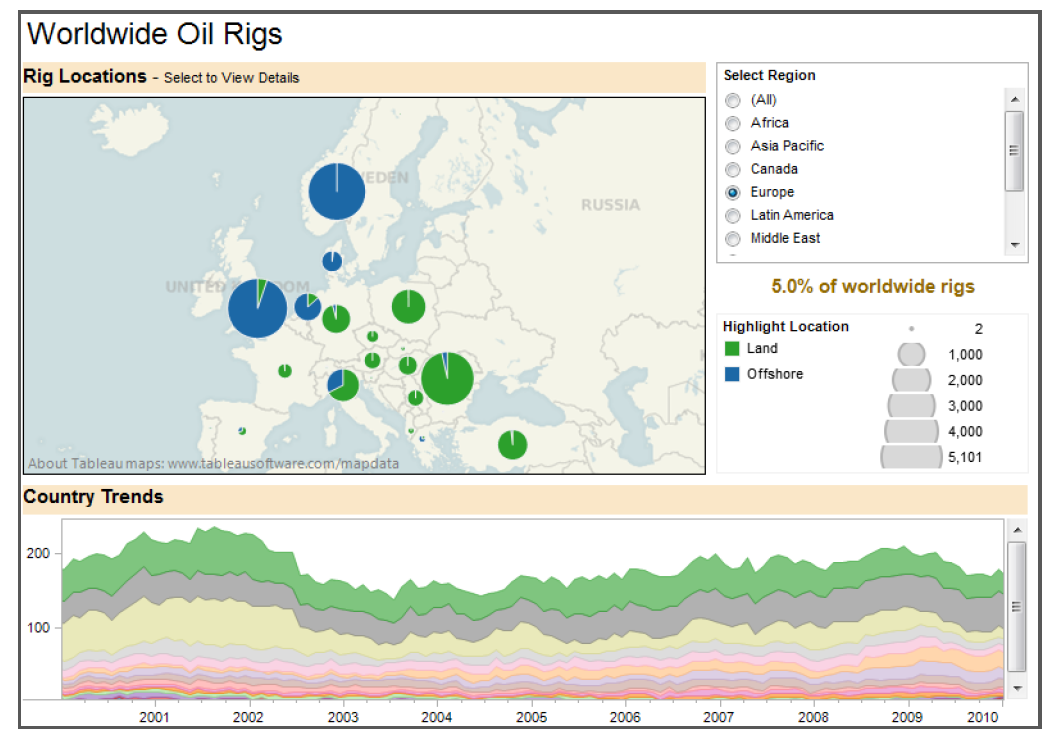
\includegraphics[width=12cm]{../../Images/02_TF_Visualisation_Pattern.png}
  \caption{The worldwide oil rigs using a combination of pie charts, a geographical map, and a line chart \parencite{OTH09}.}
  \label{fig:visualisation_pattern}
\end{figure}

Once we have selected a chart, we can tailor the chart itself. We can, for example, change the way the data markers and data labels are presented \parencite{BI09}. Figure \ref{fig:tf_good_chart} presents an example of a chart that is easy to interpret by the limited amount of information. It is consistently coloured, and the axis titles are explicit. Figure \ref{fig:tf_bad_chart} presents an example of a chart that is more difficult to interpret by the significant difference in scales, the inconsistent colouring, and the missing definitions of the axis'.

\begin{figure}[H]
\centering
  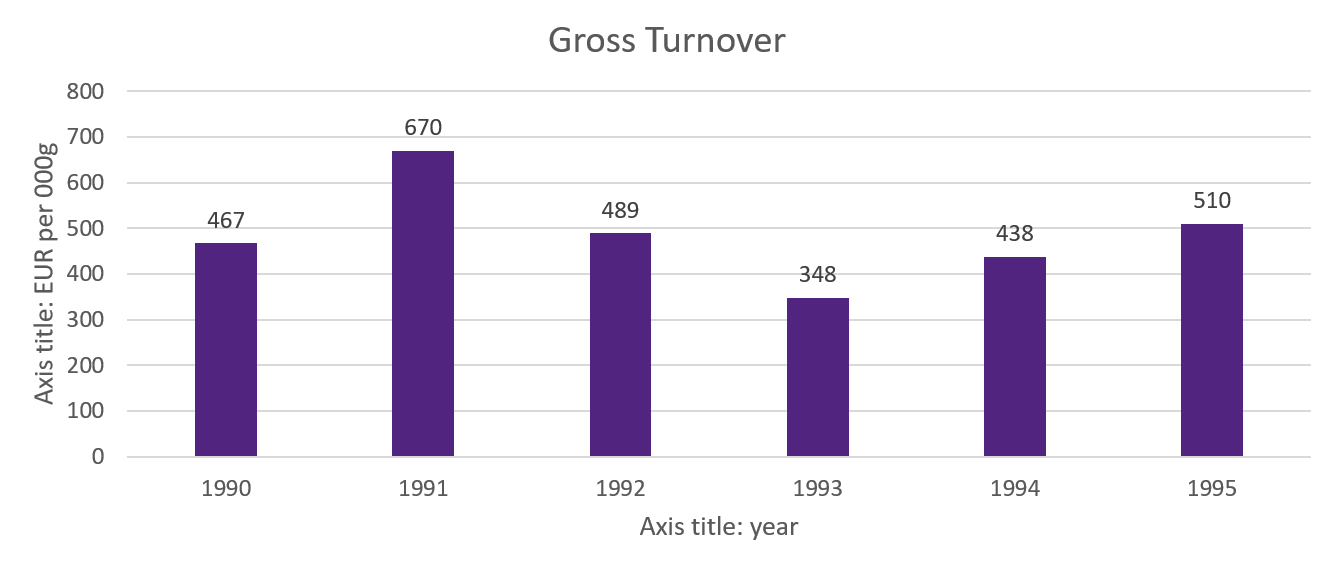
\includegraphics[width=13cm]{../../Images/02_TF/02_TF_Good_Chart.png}
  \caption{An example of a chart that is easy to interpret by the limited amount of information. It is consistently coloured, and the axis titles are explicit \parencite{BI09}.}
  \label{fig:tf_good_chart}
\end{figure}

\begin{figure}[H]
\centering
  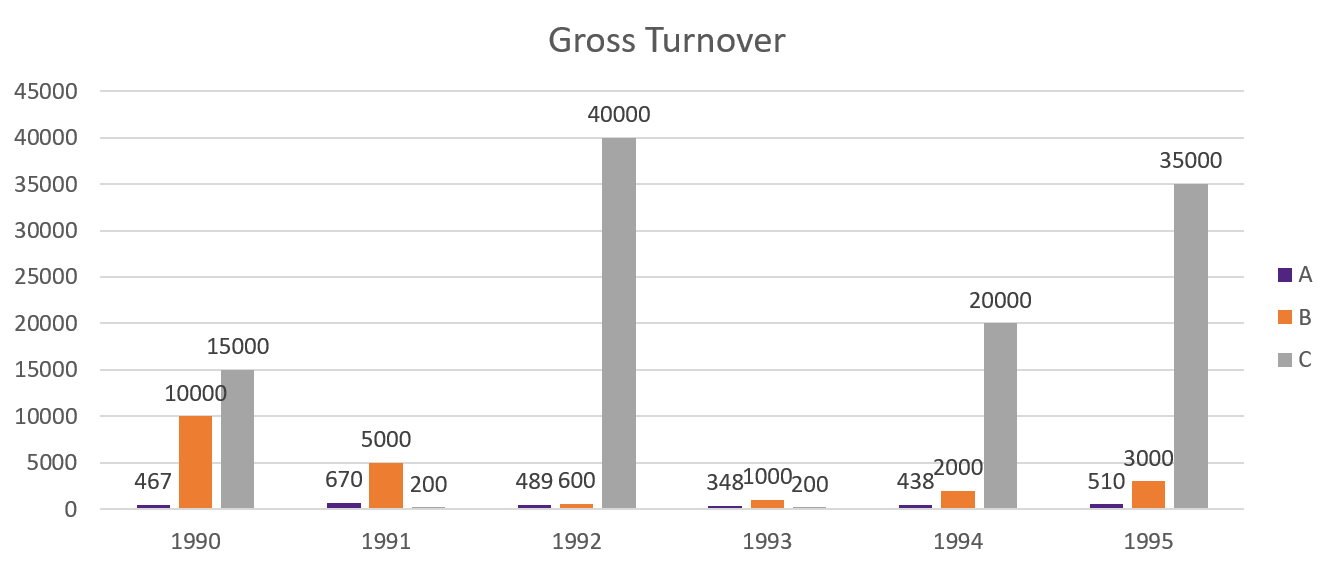
\includegraphics[width=13cm]{../../Images/02_TF/02_TF_Bad_Chart.png}
  \caption{An example of a chart that is more difficult to interpret by the significant difference in scales, the inconsistent colouring, and the missing definitions of the axis' \parencite{BI09}.}
  \label{fig:tf_bad_chart}
\end{figure}

\cite{BI09} describes best practices that are useful when we want to present information with a specific goal. For example, we should limit the usage of 3D charts as they tend to obliterate data series and are challenging to interpret. 

%=================================================================================================================================================================================================
\subsection{Generalisation}
\cite{BK03} defines a design pattern as the core of a solution for similar problems. Ontologies describe concepts on a knowledge level and focus on the structure of knowledge \parencite{SM19}. Presentation design patterns are challenging to find. However, we can interpret existing data presentation concepts like design patterns. These presentation concepts are reusable for similar problems as well.

\subsubsection{Ontology design patterns} \label{tf_odp}
\newcommand{\tfodp}{We define an ontology design pattern as an ontology configuration that effectively solves multiple problems \parencite{ODP06}.}

\tfodp

There are three types of stakeholders involved in ontology engineering \parencite{ODP02}: ontology experts, domain experts, and end-users. In general, end-users have little domain knowledge, domain experts have little ontology expertise, and ontology experts have little domain knowledge. Domain experts drive the majority of ontology development with limited involvement of ontology experts. This limited involvement might result in poor design choices \parencite{ODP02}. Ontology design patterns enable domain experts to re-use design decisions and best practices. 

\paragraph{Content ontology design patterns} \label{CODP}
A content ontology design pattern includes the generic use case, specific use-case, address logic, reference ontologies, formal relationships, sensitive axioms, and the related class diagram. This approach follows software design patterns that typically also contains a problem description, suggested solution, implementation guidelines and consequences of using the pattern \parencite{ODP07}.

\paragraph{Generic ontology design patterns} \label{GODP}
\cite{ODP06} introduced ontology design patterns in 2003. However, their adoption by ontology engineers has been slow \parencite{ODP02}. Ontology engineers have two options to use a predefined ontology design pattern:
\begin{enumerate}
\item Import the ontology design pattern as-is into an existing ontology. The import process might require some manual adjustments.
\item Manual redesign of the ontology design pattern, so it fits into the target ontology.
\end{enumerate}

The ontology design pattern clutters the ontology with information that might not be needed. Additionally, the ontology design pattern might introduce inconsistencies into the ontology related to, for example, naming conventions. Option two is very time consuming and error-prone. Generic ontology design patterns allow ontology engineers to use ontology design patterns without cluttering the existing ontologies safely. At the same time, generic ontology design patterns prevent ontology engineers from manually redesigning the ontology to fit the ontology design pattern \parencite{ODP02}. 

The Generic Distributed Ontology, Model and Specification Language (Generic DOL, or GDOL) is:
\begin{quote}\itshape
"... a meta-language that allows to define and manipulate ontologies and networks of ontologies." \parencite{ODP02}
\end{quote}

GDOL embeds OWL expressions to, for example, extend an existing OWL ontology. For example, if $A$ and $B$ are two ontologies (or instantiations of generic ontology design patterns), $A \text{ and } B$ create an intersection of the two ontologies. Additionally, generic ontology design patterns can contain parameters. The parameters allow the instantiation of customised object and property names while keeping the structure of the pattern intact. 

Ontology engineers can use the heterogeneous toolset (HETS) to implement the generic ontology design pattern into an ontology. The Heterogeneous Tool Set (HETS) interprets GDOL. HETS \emph{flattens} the ontology and generates a proper OWL ontology based on the GDOL definition. For example, HETS creates a new ontology $AB$ from the ontologies $A$ and $B$.

\cite{ODP03}, planned a Prot\'eg\'e plugin. However, there are currently no development tools available that can take care of the instantiation, extension, modification, and combination of generic ontology design patterns. 

\subsubsection{Information presentation design patterns}
Most current work focuses on the presentation of information and aims to achieve a particular goal. A prioritisation process, for example, uses a distribution chart to visualise how stakeholders have voted for an item. In contrast, the prioritisation process uses a disagreement chart to visualise the dispersion of priorities among stakeholders \parencite{BI08}. However, when we take one step back, we observe that the distribution chart is a bar chart that software product managers use to compare the priority of the different items \parencite{OTH09}. Additionally, we observe that the disagreement chart is a line chart that software product managers use to visualise the disagreement between stakeholders over the prioritised items. We consider the low-level charts as information presentation design patterns. Each chart serves as the core of a solution for similar problems. 

%=================================================================================================================================================================================================
\subsection{Software product management} \label{tf-spm}
Product lifecycle management, product requirements engineering, release planning, road mapping and the definition of a (product) vision \parencite{PM02} represent the core activities of a software product manager. Naturally, in each of these activities, a software product manager gathers knowledge and analyses information to drive a specific decision.

Product lifecycle management manages the business processes and the related information along the entire lifecycle of the product \parencite{PM14}. An alternative way of looking at product lifecycle management focuses on knowledge management. External forces play a role in product lifecycle management as well. For example, globalisation, increased complexity, shrinkage in the product life cycle (addressing the speed of change in customer needs), and environmental issues \parencite{PM15}.

Product requirements engineering defines problems based on (user) research by considering potential dependencies, assets, product lines and themes. The (technical) solution amends the problem description \parencite{PM01}. The software product manager needs to elicit and re-evaluate new requirements continuously as the market and technology evolve \parencite{PM13}.

Release planning is considered the short-term planning process that takes care of scoping and prioritising the requirements for the next product release. Prioritising requirements can be done based on multiple data inputs, including stakeholder opinions \parencite{PM01} and financial data. 

Defining the product roadmap, compared to release-planning, takes care of forecasting (market trends and technology) as well as planning (products and resources) on a mid to long-term basis \parencite{PM01}. 

The product vision is the first step in understanding why an organisation or product exists in the market. When the organisation does not understand its own business, it will start focusing on short-term issues and cost-cutting actions \parencite{PM16}. 

\subsubsection{Concepts} \label{general_concepts}
\paragraph{Insights, opportunities, challenges, and solutions}
Field research, in the context of the defined project goal, discovers problems, develops and designs solutions, tests those solutions, and confirms projects. Figure \ref{fig:ddm} presents the double diamond model and the discovery process, including field research \parencite{OTH02}.

\begin{figure}[H]
\centering
  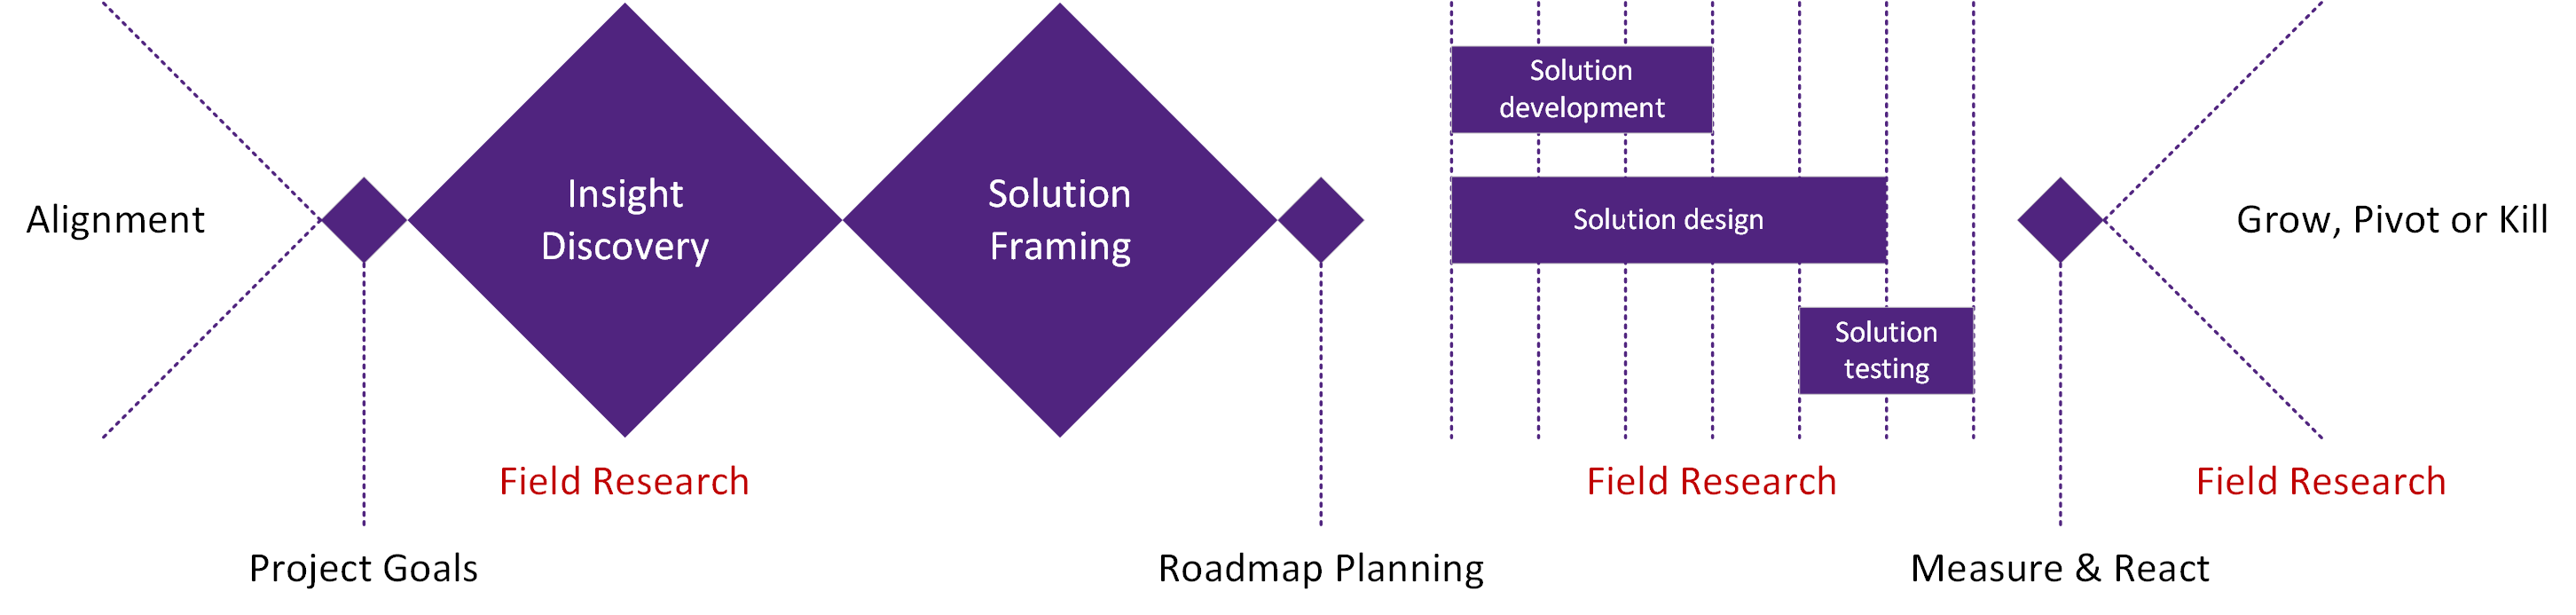
\includegraphics[width=16cm]{../../Images/DoubleDiamond.png}
  \caption{The double diamond model and shows how the discovery process embeds field research \parencite{OTH02}.}
  \label{fig:ddm}
\end{figure} 

Interesting pieces of information might surface during the field research. These pieces of information, ideally directly quoted from the source, are defined as \emph{insights} \parencite{OTH02}. An opportunity arises from a positive insight: it delights the stakeholder and motivates action. A challenge arises from a negative insight: it frustrates the stakeholder and potentially blocks the success. The product team frames a solution based on the insight. The solution goes back into the field research where a product team use new insights for further development, design, and testing. Once finished, there are three options: grow (continue), pivot (restart) or kill the project.

\paragraph{Goals and requirements} \label{gr}
Requirements prioritisation decides which requirement is most important in the context of an insight. Alternative solution selection decides the best way to address an insight. Defining what a solution exactly is and where it is coming from further supports building the common understanding.

We use the definition: \textit{'A goal is a prescriptive statement of intent the system should satisfy [...]'} \parencite{BK04} and define that a goal is equal to a solution. A software engineer needs a detailed view on a goal and slices the goal into multiple sub-goals or requirements: \textit{'A requirement is a goal under the responsibility of a single agent of the software-to-be'} \parencite{BK04}. As a result, a requirement achieves a (sub) goal. It adds customer value, even though it might not be able to address the primary goal directly. The relationship between a primary goal, potential sub-goals, and the related requirements is called a goal-model. The goal-model shows how higher-level goals are satisfied by lower-level goals (or requirements). Figure \ref{fig:gm} presents an example of a goal-model.

\begin{figure}[H]
\centering
  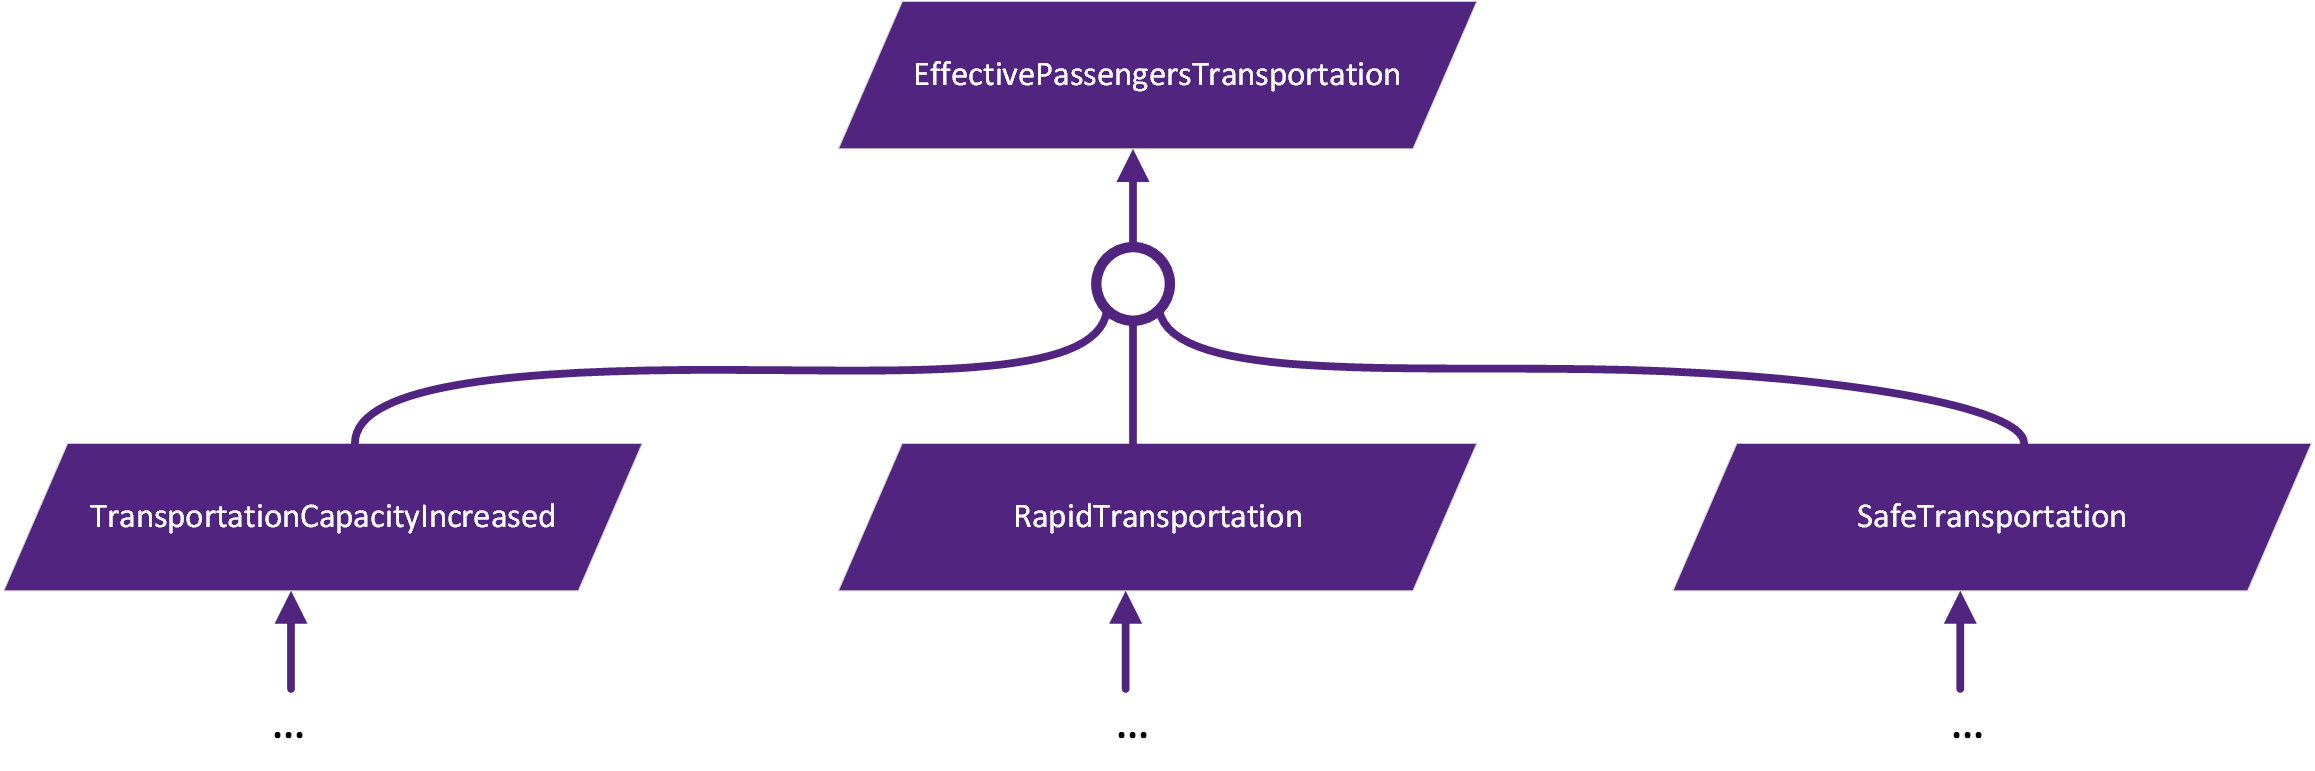
\includegraphics[width=15cm]{../../Images/GoalModel.png}
  \caption{Example of a goal-model showing the primary goal (effective passenger transportation) and its related sub-goals \parencite{BK04}.}
  \label{fig:gm}
\end{figure}

\subsubsection{Requirements prioritisation} \label{tf-val-rp}
Software is never finished: there is an endless number of requirements to improve software products or to increase its usefulness or to create a competitive advantage. Picking the right requirements can lead to great success while picking the wrong requirements can lead to utter failure \parencite{PM17}. The requirement prioritisation process focusses on a decision involving two requirements: which one is more important? 

\paragraph{An informal process that is driven by intuition} 
The requirements prioritisation process is informal and includes invisible decisions \parencite{PM20}. Continuously changing information requires that prioritisation is a continuous or iterative process. The software product manager needs to repeat this process regularly \parencite{PM22}.

The most popular technique for requirements prioritisation is the analytical hierarchical process, followed by the quality functional deployment, planning game, and binary search tree \parencite{PM29}. However, product managers hardly use these techniques, as most of them produce unreliable results or are very time-consuming. For example, the software product manager needs to manually update the prioritisation of the relevant requirements when a new requirement is introduced or deleted from the list \parencite{PM29}. 

\begin{quote}\itshape
'There is no time to analyse thousands of wishes[requirements]; much of the work is done intuitively.' \parencite{PM20}
\end{quote}

\paragraph{Criteria that influence the priority} \label{rpp_solution} 
A requirement starts with the stakeholder (typically a customer or user): an insight either motivates the stakeholder to take action (opportunity) or frustrates the stakeholder (challenge). The insight needs to contribute to achieving the product vision. Product managers should tightly couple the product vision to the value the product offers to the market \parencite{PM16}. The \emph{value} of the insight and the \emph{vision contribution} should influence the priority of the related requirements as well.

Depending on the environment, multiple stakeholders might recognise the same insight, which increases its value for the organisation. The \emph{reach} of the insight, therefore, should influence the priority of the related requirements.

A single requirement can rarely solve an insight on its own, and multiple goal-levels can be in between the insight and requirement \parencite{BK04}. The team implementing the requirement needs to define the \emph{contribution} level to the insight. At the same time, each requirement should address a small part of the insight independently. The \emph{contribution} of a requirement to each insight should influence the priority of the requirement.

From a business perspective, the product manager needs to balance the cost of developing a requirement with the business value the requirement brings \parencite{BK04}. The business value includes, for example, the costs of not implementing a requirement. The product manager should prefer requirements with high business value and a low cost over requirements with low business value and a high cost. The \emph{value} and \emph{cost} ratio should, therefore, influence the priority of a requirement.

The team implementing the requirement needs to be confident the requirement is achievable and that the requirement can address (a part of) the insight. Confidence does not only mitigate financial risks, but it also increases the efficiency of the team, and it will motivate them to implement the requirement in a way it will meet the stakeholders' expectations \parencite{PM23}. The \emph{confidence} should, therefore, influence the priority of a requirement.

\paragraph{Relative scale}
A relative scale is suitable to estimate the values of the proposed criteria \parencite{PM22}. However, a relative scale has a disadvantage as well. The scale changes when the software product manager introduces a new requirement or removes an existing requirement. This challenge can be mitigated by trying to fit requirements into a predefined scale.

\subsubsection{Alternative solution selection} \label{tf-val-as}
Each product (or product functionality) has a goal \parencite{SO03}. A goal can range from reducing the operational costs or increasing the scalability of the product. Traditional requirements engineering modelling techniques do not include the analysis of alternative solutions \parencite{SO12} that could cause the product team to select a premature solution. The outcome of this decision is a chosen solution for reaching a specific goal. Based on this decision, the team can start the implementation.

\paragraph{Selecting the best possible solution} 
An organisation starts a software project with an agreement on \emph{what} problem should be solved, \emph{why} the problem needs to be solved and \emph{who} should be involved in solving that specific problem \parencite{SO03}. For each problem, multiple (software) solutions are available. The complexity of each solution is partly defined by its functionality and by a set of non-functional requirements related to, for example, operational costs, performance, reliability, maintainability, portability, and robustness \parencite{SO06}. 

\begin{quote}\itshape
'Errors of omission or commission in laying down and taking properly into account such [non-functional] requirements are generally acknowledged to be among the most expensive and difficult to correct once the information system has been completed.' \parencite{SO06}
\end{quote}

\paragraph{Quantitative Reasoning} 
A solution describes the effect of the system-to-be on its surroundings. The product team defines the goal of the system-to-be and its composition, which might contain other (sub)goals or system requirements \parencite{SO03}. Out of the potential combinations of goals and requirements, the best solution needs to be selected. 

Product teams can use soft goals as evaluation criteria for selecting solutions among multiple alternatives \parencite{BK04}. A soft goal is a particular type of goal for which it is not possible to establish its reachability. It is possible to state a soft goal is more satisfied in alternative $a$ compared to alternative $b$. There are two options to evaluate alternative solutions using soft goals: qualitative reasoning and quantitative reasoning \parencite{BK04}. The disadvantage of qualitative reasoning is that the propagation rules have a high probability of generating an inconclusive outcome that does not make it suitable for this study. 

\begin{quote}\itshape
'The aim is to determine, for each alternative, a [...] degree of satisficing of the top-level soft-goals in the goal refinement graph; the option with the best degrees of satisficing is then selected.' \parencite{BK04}
\end{quote}

Qualitative reasoning assesses the positive or negative contribution of a solution to the soft goal: the product team needs to score each potential solution against the soft goal. A score $x$ means that the solution contributes to the soft goal for $x$\% \parencite{BK04}. Figure \ref{fig:sg} presents the goal \emph{optimal track usage}. Optimal track usage is essential for the busy rail network in, for example, Japan. The system-to-be needs to achieve this (soft) goal while taking safe transportation into account. There are two potential solutions for avoiding a train collision: avoiding trains to enter the same rail block and maintaining a worst-case stopping distance. Assuming the worst-case stopping distance is shorter than the entire rail block, this is the chosen solution. It allows maximising the rail block usage while avoiding train collisions.

\begin{figure}[H]
\centering
  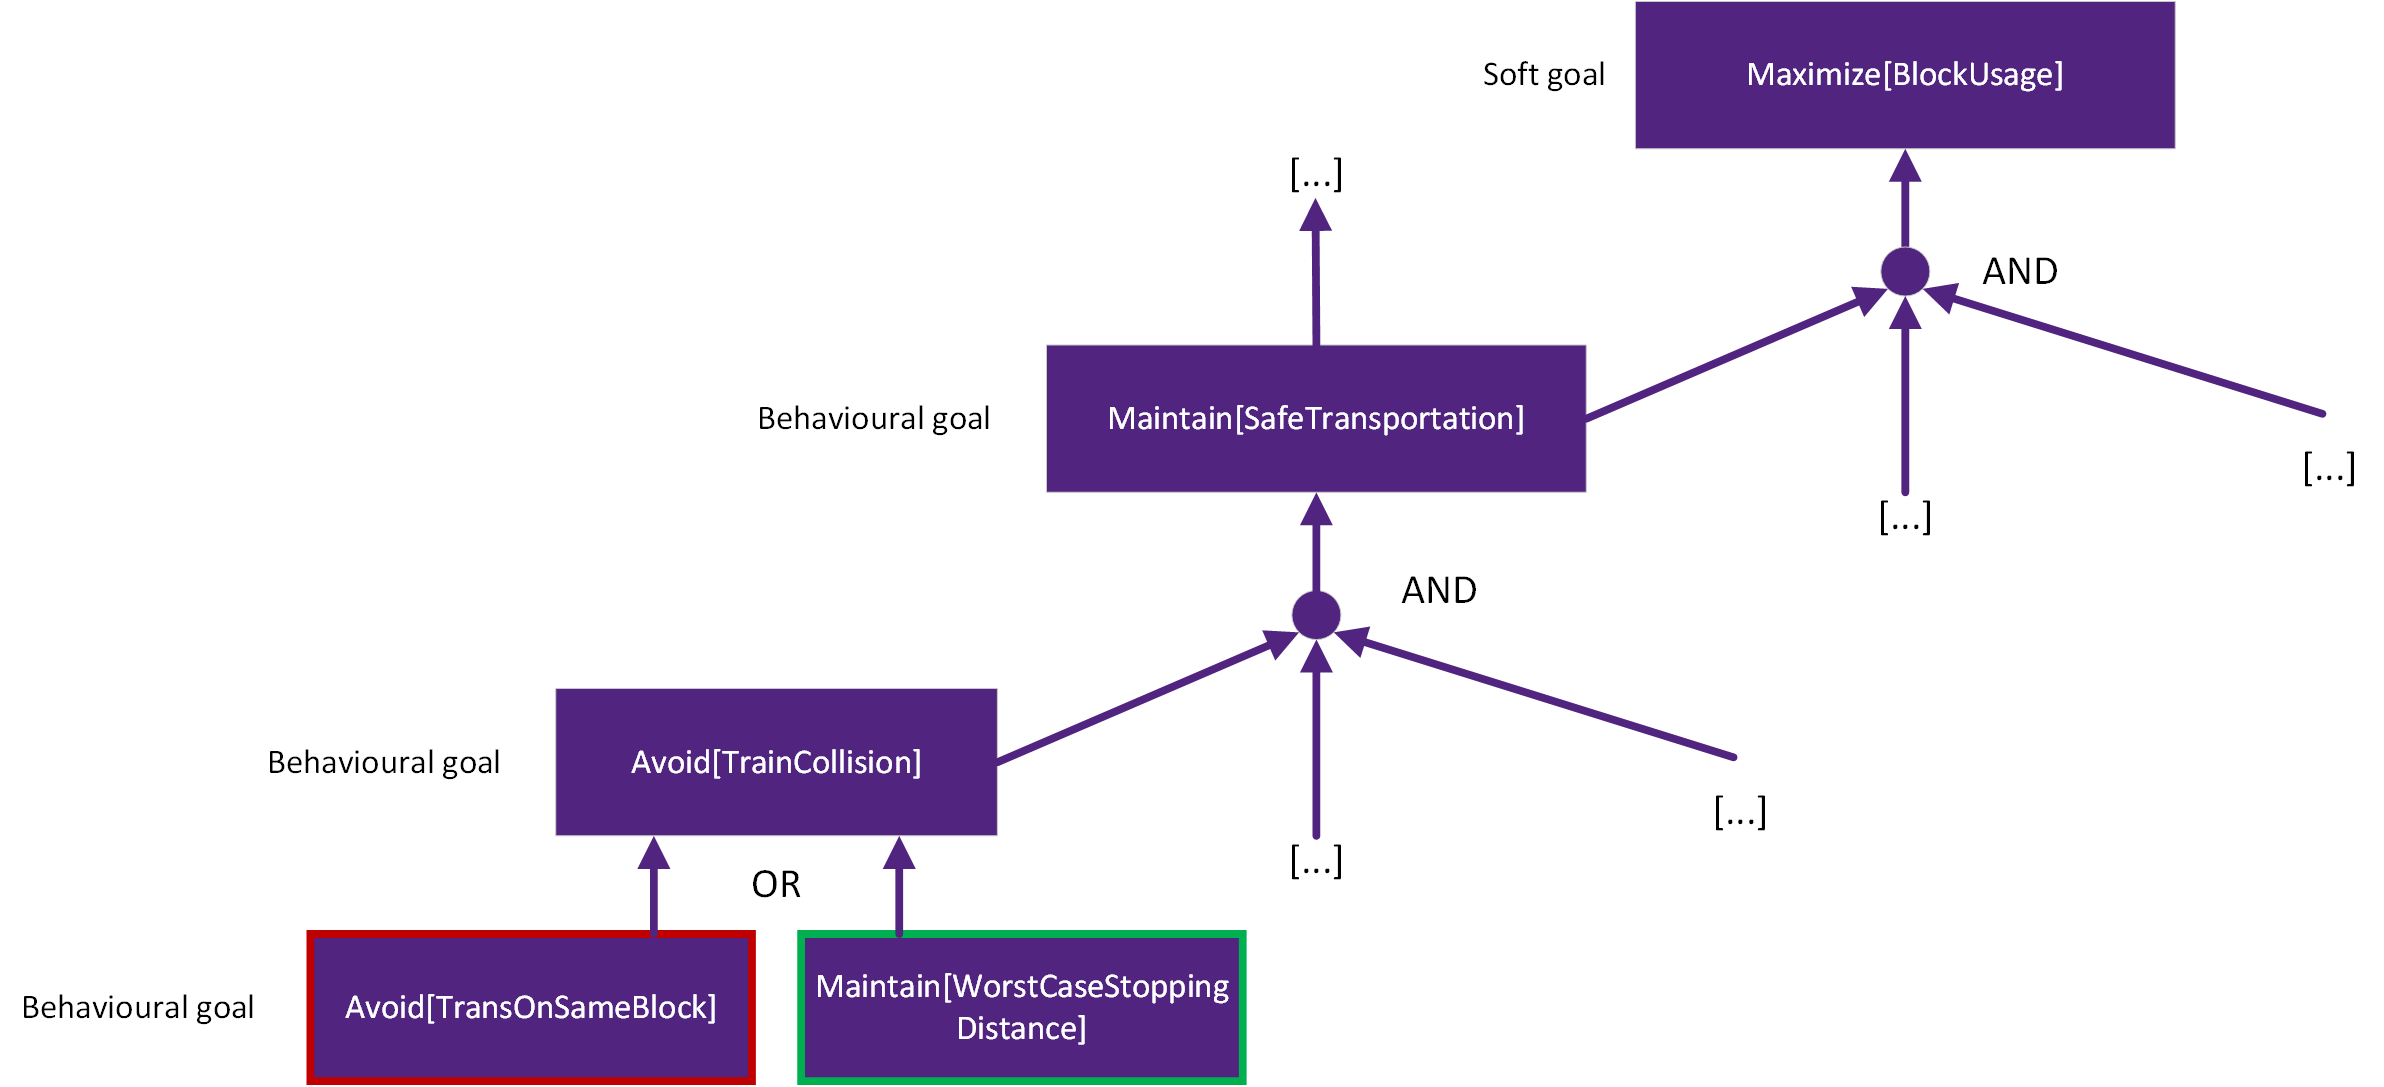
\includegraphics[width=17cm]{../../Images/SoftGoal.png}
  \caption{The selection of a solution for the efficient usage of a railway system based on higher-level soft goal \parencite{BK04}.}
  \label{fig:sg}
\end{figure}

We assign each soft goal with a weighted significance when the system-to-be needs to achieve multiple soft goals. \cite{BK04} proposes to use equation \ref{eq:totalScore} to calculate the total score that sums up the individual scores of the solutions and weighs them based on relative importance.

\begin{equation} \label{eq:totalScore}
totalScore(solution)=\sum_{soft\text{-}goal} (Score(solution,soft\text{-}goal) \times Weight(soft\text{-}goal)) 
\end{equation}

Equation \ref{eq:totalScore} calculates the value of the combined solution and soft goal by multiplying the weighted significance of a soft goal with the score of the solution. The sum of the values assigned to a solution determines the evaluation of the solution (equation \ref{eq:totalScore}). Table \ref{table:itass_example} shows an example where the equation prefers to maintain the $WorstCaseStoppingDistance$ over avoiding $TrainsOnSameBlock$ \parencite{BK04}.

\begin{table}[H]
\centering
\caption{Example of the usage of equation \ref{eq:totalScore} in which $Maintain[WorstCaseStoppingDistance]$ is preferred over $Avoid[TrainsOnSameBlock]$.}
\begin{tabular}{| p{4cm} | p{2cm} | p{4cm} | p{5cm} |}
\hline
\rowcolor{document}
\color{documentText}Soft-goal & \color{documentText} Significance weighting & \color{documentText}Maintain [WorstCaseStoppingDistance] & \color{documentText}Avoid [TrainsOnSameBlock] \\
\hline
Maximize[BlockUsage] & 0.50 & 0.90 & 0.30 \\
\hdashline
Soft goal 2 & 0.30 & 0.50 & 0.90 \\
\hdashline
Soft goal 3 & 0.10 & 0.80 & 0.30 \\
\hdashline
Soft goal 4 & 0.10 & 0.50 & 1.00 \\
\hline
Total & 1.00 & 0.73 & 0.55  \\
\hline
\end{tabular}
\label{table:itass_example}
\end{table}

% Summary of the theoretical framework.
\subsection{Conclusion} \label{tfconclusion}
Decision-makers use more than written or scientific sources to make their decisions. The values and experience the decision-maker and organisation bring influence the decision. A decision is always time-critical. There is a balance between elaborating on the available information to increase the maturity-level and accepting the current maturity-level of the available information and making the decision. The perfect decision does not exist. There is always some prematurity in the information decision-makers have access to and limited time to increase the maturity-level. 

\begin{center}
\large\color{document}{When decision-makers know the maturity-level, they can explicitly decide to spend more time to elaborate on the information or to make the decision based on the current maturity-level.} \\
\end{center}

The Semantic Web offers capabilities to validate if the information stored in an ontology is consistent, to classify information, and to detect missing information. We see an opportunity to bridge these capabilities to detect, for example, if specific information is reproducible or meeting a certain consensus-level. 

Design patterns exist in different flavours but have one thing in common: they solve a general problem. Generic ontology design patterns can generalize a data structure. We have not been able to find design patterns for other Semantic Web technologies, for example, SWRL rules or SHACL constraints. Information presentation design patterns do not seem to exist explicitly. However, we can extract information presentation patterns from existing scientific and commercial sources. 